% 06.1.2. ESTIMACIONES GLOBALES DE TAMAÑOS Y ESFUERZOS INICIALES
%----------------------------------------------------------------------------------------

\paragraph{} Se muestra en la figura \ref{fig:6121} los tiempos que se han asignado a las diferentes tareas. En esta figura se muestran las horas concretas que se estimaron al principio del proyecto. Más adelante se mostrara cuantas horas reales se invirtieron en cada apartado.

\begin{figure}[h!]
\centering
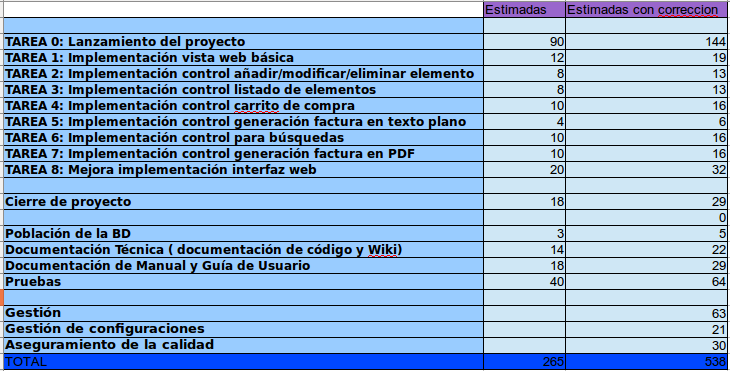
\includegraphics[width=0.95\textwidth]{img/6121}
\caption{Estimación esfuerzos totales}
 \label{fig:6121}
\end{figure}

\paragraph{} Se muestra en la figura \ref{fig:6122} las horas asignadas a cada una de las tareas. Se puede ver que las partes más costosas son sobre todo el lanzamiento del proyecto,gestión y pruebas.Implementación se llevaría otra de las grandes partes del proyecto, pero al estar dividida en subtareas parece que ocupe un tiempo menor del que en realidad lleva.

\begin{figure}[h!]
\centering
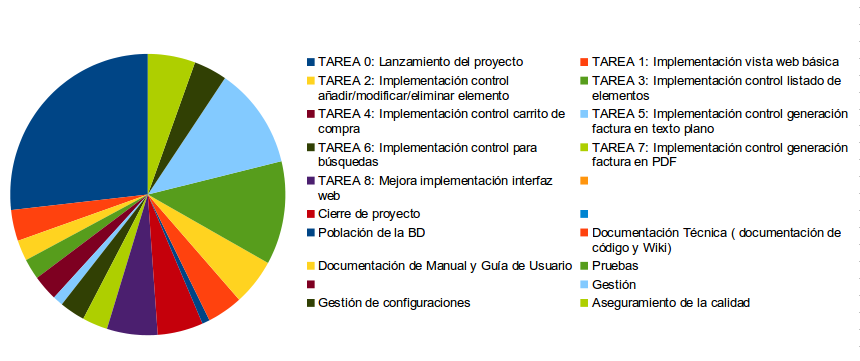
\includegraphics[width=0.95\textwidth]{img/6122}
\caption{Gráfica esfuerzos totales}
 \label{fig:6122}
\end{figure}